\begin{figure}[htb]	
\center%6.3
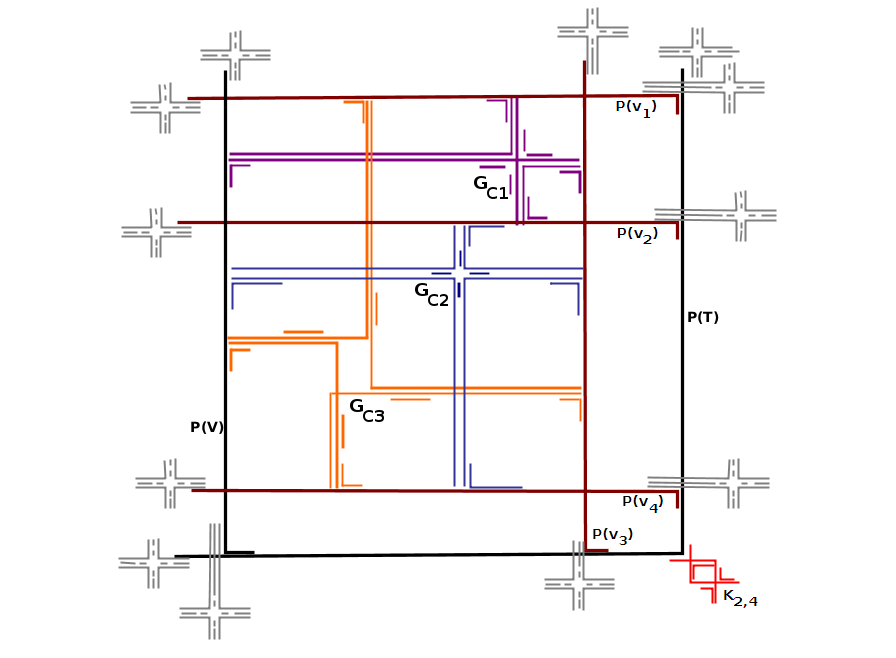
\includegraphics[width=1\textwidth]{./img/formulaGFCompletaSBPO3diferentes2.png}
\caption{The $B_{1}$-EPG-Helly representation to gadget $G_{F}$ of the Figure~\ref{fig:exemploGrafoGF}.%, to formula $F=(x_1+ x_2+ x_3) \wedge  (x_2+ x_3+ x_4 )\wedge  (x_1+ x_3+ x_4 )$. 
 The gadget's clause $G_{c_1}$ represented by false pie, the gadget's clause $G_{c_2}$ represented by true pie, and the gadget's clause $G_{c_3}$ represented by frame.}
\label{fig:grafoFormula}
\end{figure}
